\chapter{Evaluation}
\label{ch:evaluation}

This chapter discusses three different experiments that are conducted to check for effectiveness and efficiency of RDF-Doctor.
First experiment checks the effectiveness of RDF-Doctor against set of test cases provided in~\cite{TurtleTests:Online}.
In the second experiment, a random number of errors is generated using a Poisson Distribution for a period of eight instances of time while a Uniform Distribution randomly selects types of errors for each instance of time, respectively.
%number generators for a period of time of 8 time instances to simulate a couple of syntax errors, produced by an ontology user, 
Finally, the efficiency of RDF-Doctor is measured when both, the number of errors and the size of ontologies are changed. 

In the following sections, three experiments designed to evaluate RDF-Doctor are presented. 
Each section describes a particular experiment by giving its objective, presenting the followed procedure, and discussing the achieved results.

\section{Experiment Configuration}

All experiments are run on a Linux Ubuntu 18.04 machine with a 4th Gen Intel Core i5-4300U CPU, 3MB Cache, 2.90GHz with 8GB RAM 1333MHz DDR3. 
RDF-Doctor is implemented using Java version 9. 
ANTLR framework version 4.7.1 is used to build the internal parser in RDF-Doctor.%, as well, as an imported library for compiling and running of it.  

\section{Validating with RDF Suite Test} 
In this experiment, RDF-Doctor was validated against RDF Suite Test, specifically Turtle serialization. 
%Next text discusses the objective, shows the procedure, and finally, presents and discusses the result.  

\subsection{Objective}

There exists a number of Test Suites for each RDF serializations which are recommended by W3 Consortium (W3C) in ~\cite{TurtleTests:Online}.
%The evaluation phase starts with where a Test Suite defined in the Turtle serialization. 
These Test Suites can be used to check for the proficiency of a parser with respect to a certain serialization.% can be validated with these files found in a corresponding Test Suite. 
Therefore, the target of this experiment is to measure the proficiency of RDF-Doctor while testing with the W3C Turtle Test Suite.

\subsection{Procedure}

Files at \cite{TurtleTests:Online} were prompted to validate a parser that parses a Turtle serialization, hence, it was used to test RDF-Doctor. 
Metrics of the experiment are both Precision and Recall, donated by equation \ref{eq:1} and \ref{eq:1} sequentially. The former measures the percentage of errors which correctly flagged as syntax errors, while the latter calculates the percentage of actual syntax errors which correctly recognized. Total number of files at \cite{TurtleTests:Online} is 275, divided to parts: files include  correct syntaxes; and files contain incorrect syntaxes, the latter is represented with 65 files, and the remaining are related to the former, as demonstrated by Table \ref{tab:TurtleSuit}. 
 
\begin{table}[]
\centering
\begin{tabular}{|l|l|l|l|}
\hline
\begin{tabular}[c]{@{}l@{}}Error Type Classification \end{tabular} & Detected & \begin{tabular}[c]{@{}l@{}}Not detected\end{tabular} & Total \\ \hline
 Escape Characters              &      0    &    4 &   4  \\ \hline
 Bad Keywords             &      5   &    0 &   5  \\ \hline
 Bad Literals with langTag             &      2   &    0 &   2  \\ \hline
 Bad Local Name-space in IRI             &      2   &    3  &   5  \\ \hline
 Bad Namespace in IRI             &      2   &    0 &   2  \\ \hline
 N3 Extra             &      11   &    1 &   12  \\ \hline
 Bad Namespace in Directives             &      2   &    0 &   2  \\ \hline
 Bad Number as a Literal             &      5   &    0 &   5  \\ \hline
 Bad Directives             &      4   &    0 &   4  \\ \hline
 Bad Strings             &      6   &    1 &   7  \\ \hline
 Bad Structures            &      12   &    0 &   12  \\ \hline
 Bad IRI            &      2   &    3 &   5  \\ \hline
 Total            &      53   &    12 &   65  \\ \hline
\end{tabular}
\caption{\textbf{Evaluation of RDF-Doctor against detection of incorrect syntactic forms in Turtle Test Suite \cite{TurtleTests:Online}.} The test focuses on the files, including  an incorrect Turtle syntax,  ”Detected” in pointed to recognized syntactic forms as incorrect forms with releasing corresponding error messages, but ”Not detected” specifies incorrect syntactic forms which are not recognized and might generate false positives.}
\label{tab:detection}
\end{table}

\subsection{Result and Discussion}

The test drives the result when dealing with either correct or incorrect Turtle syntax. Thus, correct syntaxes should be recognized as correct, similarly in case of incorrect syntaxes plus exception errors should be fired.  However,  the test result in Table \ref{tab:TurtleSuit} shows recognizes mostly of correct syntaxes with 88\%, while the remaining 12\% RDF-Doctor are not recognized and it consider them as errors. In the meanwhile, when dealing with incorrect syntaxes, again, Table \ref{tab:TurtleSuit} provides that 81,5\% of files included incorrect syntaxes are detected and an error message was fired for each one of them, the rest 17,5\% go without being identified as incorrect forms, as well as no errors were fired.



\begin{table}[]
\centering
\begin{tabular}{|l|l|l|l|}
\hline
\begin{tabular}[c]{@{}l@{}}File Content \end{tabular} & Detected  & Not detected & Total \\ \hline
 Correct Syntax              &      185    &      25  & 210 \\ \hline
 Incorrect/Bad Syntax              &      53    &    12  & 65 \\ \hline
 Total            &      238   &       37 & 275  \\ \hline
\end{tabular}
\caption{\textbf{Evaluation summary of RDF-Doctor for both correct and incorrect syntactic forms when validating with Turtle Test Suite \cite{TurtleTests:Online}.} "Detected" for Correct Syntax means that RDF-Doctor is able to recognize them as correct syntactic forms, whereas, for those which are not correctly recognized classified under "Not detected", similarly, "Detected" in Incorrect/Bad Syntax referred to recognized syntactic forms  as incorrect forms with releasing corresponding error messages, but "Not detected" specifies  incorrect syntactic forms  which are not recognized and might generate false positives.}
\label{tab:TurtleSuit}
\end{table}
\begin{figure}[ht]
\begin{center}
		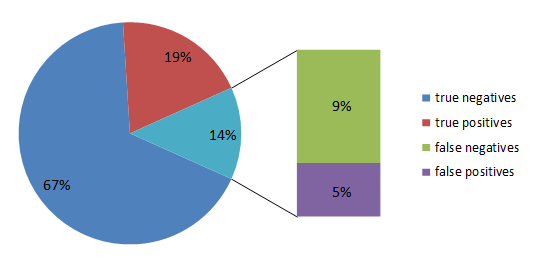
\includegraphics[scale=0.8,angle=0]{images/Experiment01.png}
		\caption{\textbf{RDF-Doctor evaluation with Turtle Test Suite \cite{TurtleTests:Online}.} Each file in \cite{TurtleTests:Online} was classified of having a syntax error or not and then the final result was grouped into 4 categories: true positives (files with syntax errors are correctly identified); false positives (files without syntax errors are incorrectly identified); false negatives (files with syntax errors are incorrectly rejected); true negatives (files without syntax errors are correctly rejected).}
		\label{Fig:Experiment01}
\end{center}
\end{figure}

For evaluation, the precision and recall are computed using the equations \ref{eq:1} and \ref{eq:2} respectively.  
\begin{align} 
   Precision=  \frac{t_p}{t_p+f_p}\,;\qquad
\qquad\parbox{4.0cm}{\footnotesize$\begin{aligned} t_p &= \text{ number of true positives}\\[-1.0ex] f_p &= \text{ number of false positives}\end{aligned}$}
   \label{eq:1}
\end{align}
\begin{align}
   Recall =  \frac{t_p}{t_p+f_n} \,;\qquad
\qquad\parbox{4.0cm}{\footnotesize$\begin{aligned} t_p &= \text{ number of true positives}\\[-1.0ex] f_n &= \text{ number of true negatives}\end{aligned}$}
   \label{eq:2}
\end{align}



\section{Validating with Random Syntax Errors Generation}
RDF-Doctor is being validated with injected syntax errors in random. What follows is a details of this experiment.
\subsection{Objective}
To get rid of the generated bias, this experiment uses both Poisson distribution and uniform random number generation methods. It also assumes a naive user editing an RDF input data, found in an environment similar to the one in Figure \ref{Fig:Motivation} and he is mistakenly generating some  syntax errors. Then, the inserted syntax errors evaluate the quality of RDF-doctor.


\subsection{Procedure}
 In this experiment, a naive user who is working on on RDF input data for 8 time instances and each one hour he is making a text change (insert/modify/delete) before submission to RDF-Doctor for parsing is simulated. The average number of making syntax errors per time interval is represented by a parameter $\lambda$. For example, if   $\lambda$ = 5, it means that five syntax errors are occurred per hour.  As an input for a Poisson distribution, 10 syntax errors per instance of time was supplied. Hence, for each instance of time we calculate value of $\lambda$, then the output value drives how many number of syntax errors are entitled for that instance of time.
 
 	\begin{figure}[ht]
	\begin{center}
		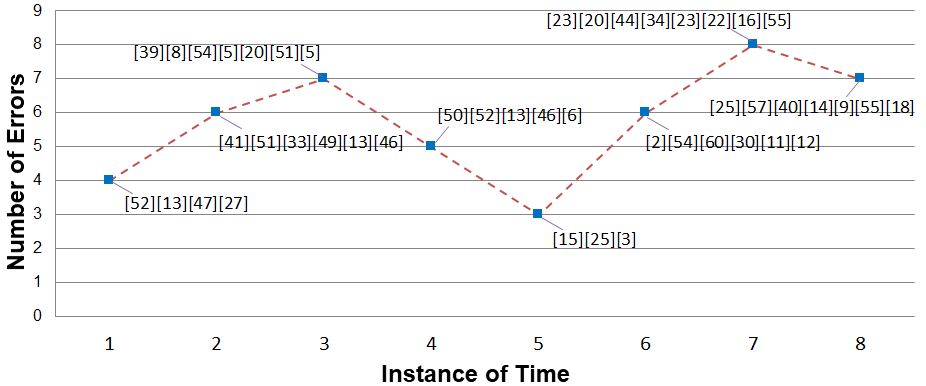
\includegraphics[scale=0.45,angle=0]{images/Experiment02-01.png}
		\setlength\belowcaptionskip{-5mm}
		\caption{\textbf{Random syntax errors distribution.} Number and types of syntax errors between brackets for a user in an interval of 8 instances of time. A Poisson  distribution with $\lambda$ = 5 models an average of 5 syntax errors per instance of time. Each instance of time shows value of $\lambda$, assuming the user can generate [1-10] syntax errors per instance of time. Also, a uniform random number generator computes type of errors from [1-61] syntax errors in Table \ref{tab:syntaxErrorCate}. For example, at the 5\textsuperscript{th} instance of time, $\lambda$ = 3, then 3 types of syntax errors are randomly generated.} 
		\label{Fig:experiment2}
	\end{center}
\end{figure}

 Next, Those syntax errors are arbitrarily selected from the type of errors range [1-61], drawn by rows of Table \ref{tab:syntaxErrorCate}. Beside locations of injected syntax errors were controlled in a semi-random method, using the uniform random number generation to get a suggested line number if this location can be a correct location for such an error, otherwise, it can be nearby of the suggested line number on the top lines of the input file, such as Prefix and Base directives.   

	\begin{figure}[ht]
	\begin{center}
		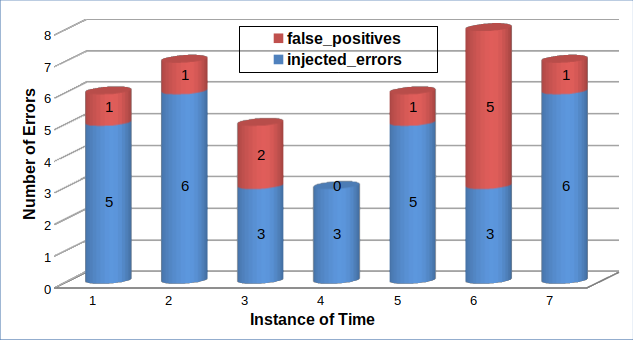
\includegraphics[scale=0.6,angle=0]{images/Experiment02-02.png}
		\setlength\belowcaptionskip{-5mm}
		\caption{\textbf{RDF-Doctor evaluation of error detection when syntax errors are randomly distributed.} For every instance of time, result shows number of errors between the injected one which were correctly detected by RDF-Doctor with giving corresponding error messages, pointed with "detected", and those one which were undetected and unrecognized by RDF-Doctor, referred as "undetected".} 
		\label{Fig:Experiment02-02}
	\end{center}
\end{figure}
\subsection{Result and Discussion}
RDF-Doctor shows promising result in Figure \ref{Fig:Experiment02-02}. In half of the time instances, only one syntax error was missed and goes unrecognized, the remaining were detected. The rest of the times instances show zero or few errors, except the time instance number 6\textsuperscript{th}, shows 5 undetected syntax errors, this can be due to fall most of the unrecognized syntax errors in this time instance since the insertion of the syntax errors was done randomly.  

	\begin{figure}[ht]
	\begin{center}
		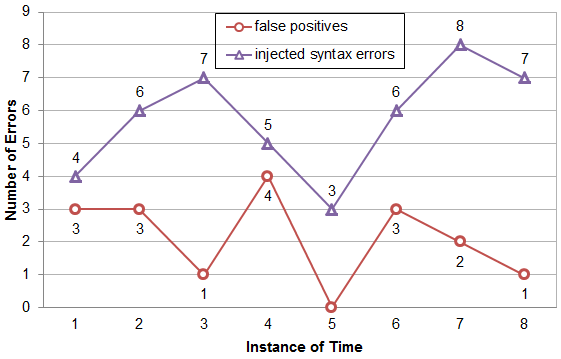
\includegraphics[scale=0.7,angle=0]{images/Experiment02-03.png}
				\setlength\belowcaptionskip{-5mm}

		\caption{\textbf{Result of false positives during RDF-Doctor validating with randomly distributed syntax errors.} For each time instance, when number of syntax errors are inserted at random, that may result in false positives since one of the unrecognized syntax errors can be in-between those inserted ones.} 
		\label{Fig:Experiment02-03}
				\setlength\belowcaptionskip{-5mm}
		\setlength\abovecaptionskip{0mm}
	\end{center}
\end{figure}
Figure \ref{Fig:Experiment02-03} ex habits the comparison of the number of the injected syntax errors versus the number of false positives of this experiment. The result presents a high number of false positive, but this again due the probability of existing one or more of the unrecognized syntax errors. We think that with the new version of ANTLR this issue can be solved or by optimizing RDF-Doctor to handle this internally in another level of syntax error detection beside the error production rules in the grammar. 


\section{Impact of Number of Errors and Volume}
In last experiment, behaviour and  performance RDF-Doctor is being evaluated when a number of syntax errors and a volume of ontologies are changed. Details are shown in the following.  
\subsection{Objective}

In order to study the behaviour and the performance of RDF-Doctor, this experiment was performed. We are studying the effect of growing of number of syntax errors, as well as, the size of ontologies when it is changed. 


\subsection{Procedure}
Two types of ontologies are used: small; and medium size. For the former, FOAF  (an abbreviation form of friend of a friend) Vocabulary\footnote{http://www.foaf-project.org/} was used, it is a small ontology with volume of about 23.3 Kbyte, including people-related terms. Whilst the latter made use of the ontology  of DBpedia schema\footnote{https://wiki.dbpedia.org/develop/datasets/dbpedia-version-2016-10}, version 2016-10, with volume of about 4.1 Mbyte, including meta-data about all contained datasets of DBpedia. Both datasets were used 3 times and for one time 10, 30, 61 syntax errors were randomly  injected using the same procedure of uniform random generation. Additionally, to evaluate the performance of RDF-Doctor, same 6 of the datasets were parsed for 5 times to get the average of processing time  

 
\subsection{Result and Discussion}
Figure \ref{Fig:Experiment03-01} drives the impact of number of errors and the volume size. When introducing 10 syntax error, 9 out 10 were detected and one was not detected for both FOAF and DBpedia. 25 out 30 injected syntax errors in FOAF and 26 out 30 injected syntax errors in DBpedia were detected, the rest are undetected. Subsequently, 61 syntax errors were inserted 6 and 11 syntax errors go undetected in FOAF, DBpedia, respectively, the remaining are detected with expressive error messages to help users in resolving such errors. 
\begin{figure}[ht]
\begin{center}
		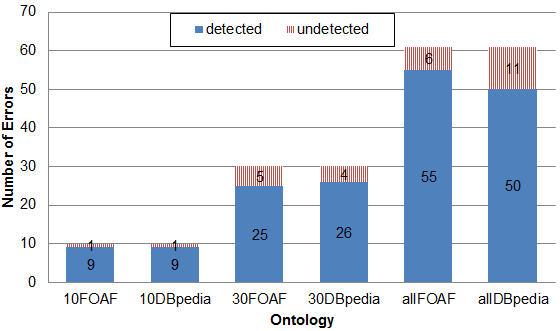
\includegraphics[scale=0.55,angle=0]{images/Experiment03-01.png}
				\setlength\belowcaptionskip{-5mm}

		\caption{\textbf{Impact of number of errors and volume on RDF-Doctor.} FOAF, and DBpedia ontologies were used to evaluate RDF-Doctor, 10foaf, 30foaf, allfoaf are datasets of FOAF ontology, including with 10, 30, 61 random syntax errors, respectively, same is applicable for DBpedia. Detected errors are the errors which were properly identified by RDF-Doctor and the matched error messages were released, while undetected errors are those which not correctly recognized.}
		\label{Fig:Experiment03-01}

\end{center}
\end{figure}


Another essential point is number of false positives were shown in the result, as it is demonstrated  by Figure \ref{Fig:Experiment03-02}. Clearly, it can be seen that the false positives  are incremented while raising of the number of syntax errors, that comes as consequence of increasing number of unrecognized syntax errors, then the parser tries to recover from such errors by adding or removing some tokens which produces more and more false positives.   




\begin{figure}[ht]
\begin{center}
		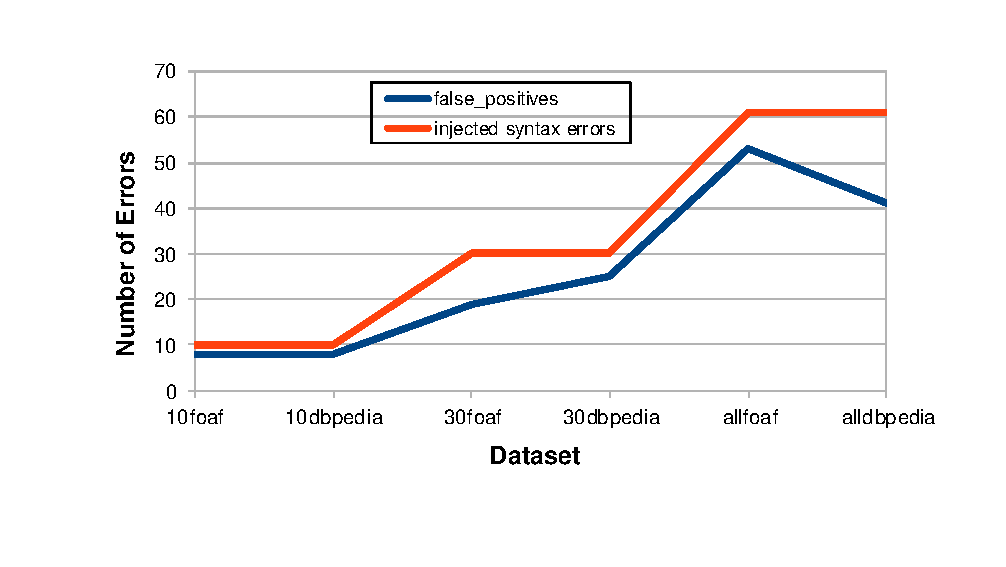
\includegraphics[scale=0.8,angle=0]{images/Experiment03-02.pdf}
		\setlength\belowcaptionskip{-5mm}
		\setlength\abovecaptionskip{-10mm}
		\caption{\textbf{Result of false positives when number of errors and volume sizes are varied.} Undetected errors generate false positive errors and when the number of errors increase, the false positives are comparably increased.}
				\label{Fig:Experiment03-02}
\end{center}
\end{figure}

Due to the need to measure the RDF-Doctor performance, Figure \ref{Fig:Experiment03-03} was presented. it summaries the impact of both number of errors and volume on RDF-Doctor performance, where numbers of errors has no influence on the performance, as the processing time similar result in either FOAF or DBpedia while changing number of errors. In the meanwhile, volumes has a high impact on the performance, since  DBpedia  takes about 29000 ms in average to be processed, whereas, FOAF was parsed in about 2000 ms.   

To conclude this experiment, It can be seen that number of error detection is promising, more than 90\% of injected syntax errors were detected, as Figure \ref{Fig:Experiment03-01} talks. Also, number of false positives can be improved if RDF-Doctor recognized those undetected errors by either do more laboratory works to match those patterns or may with the new versions of ANTLR library.  
%talk about the correction of errors #numbers 
\begin{figure}[ht]
\begin{center}
		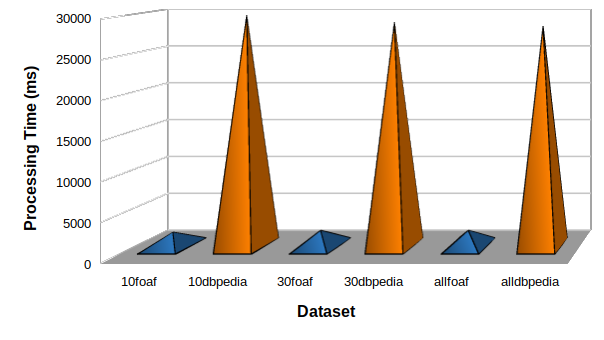
\includegraphics[scale=0.7,angle=0]{images/Experiment03-03.png}
		\setlength\belowcaptionskip{-5mm}
		\setlength\abovecaptionskip{0mm}
		\caption{\textbf{RDF-Doctor performance evaluation when number of errors and volume sizes are varied.} Performance is measured with the processing time in (ms) of FOFA ontology (23.3 Kbyte) and DBpedia ontology (4.1 Mbyte) with 10, 30, and 61 (refereed as all) injected syntax errors.}
				\label{Fig:Experiment03-03}

\end{center}
\end{figure}
